\chapter{Ambiente di analisi}
Lo scopo dell'analisi \`e quello di effettuare misure di \emph{dependability} sul software che implementa SFA (\emph{SensorFusionLib}), attraverso una campagna di \emph{fault injection}.\\*
Il sistema su cui verr\`a effettuata l'analisi \`e un'architettura \texttt{x86} equipaggiata con il sistema operativo \texttt{Windows 7}.\\*
In questo capitolo si descrive l'ambiente di analisi mappando gli strumenti teorici, noti dalla letteratura ed esposti in 1.3, su quelli effettivamente utilizzati.\\*
Il \emph{target component} \`e la libreria \emph{SensorFusionLib}.
\section{Il tool di analisi}
Il \emph{tool} di analisi utilizzato \`e un software denominato \emph{RailTrackTool} (RTT).\\*
RTT \`e un software appositamente progettato per valutare le performance di SFA, effettuare campagne di \emph{monitoring} e \emph{fault injection}. Esso funge da \emph{controller} ed integra al suo interno il \emph{load generator}, l'\emph{injector} e il \emph{monitor}.
\subsection{Load Generator}
Il \emph{load generator} \`e lo strumento preposto a fornire il \emph{workload} al sistema.\\*
In quest'applicazione, SFA viene alimentato dalle misure campionate da IMU, Odometro e GPS, installati a bordo di un treno che si muove lungo una traccia ferrotramviaria.\\*
Un ulteriore input \`e rappresentato dalle informazioni geografiche della traccia.\\*
\`E stata realizzata una libreria software (\emph{SynthDataGen)} in grado di generare le misure che verosimilmente verrebbero campionate nel sistema reale, in base ai riferimenti geografici della traccia.\\*
\begin{figure}[h]
	\centering
	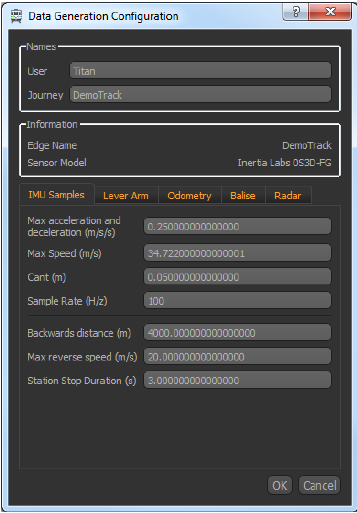
\includegraphics[width=0.7\linewidth]{img/isdg}
	\caption{Interfaccia utente verso \emph{SynthDataGen}}
	\label{fig:datagenerationconfig}
\end{figure}
\FloatBarrier
L'osservatore ha la possibilit\`a di definire:
\begin{itemize}
	\item Le caratteristiche tecniche dei sensori: rumore di misura \cite{measnoise} e frequenza di campionamento;
	\item La velocit\`a massima che il treno pu\`o raggiungere;
	\item L'accelerazione massima.
\end{itemize}
Il rumore di misura viene fornito al \emph{load generator} come:
\begin{itemize}
	\item Matrice di covarianza, per campionamenti multivariati (IMU);
	\item Varianza, per campionamenti univariati (Odometro).
\end{itemize}
Quando viene generato un possibile campionamento, il valore prodotto viene perturbato di una quantit\`a pari al valore generato da una \emph{distribuzione gaussiana} a media nulla e varianza (o covarianza) specificata.\\*
\emph{SynthDataGen} non supporta la generazione di campionamenti GPS. Questo accade poich\`e i valori campionati da un GPS sono caratterizzati da un rumore di misura che non rispetta una distribuzione gaussiana, infatti la \emph{reliability} delle informazioni GPS dipende da parametri non predicibili come il numero di satelliti attualmente in grado di fornire la posizione al ricevitore.  \cite{gpsdarkarea}
\begin{figure}[h]
	\centering
	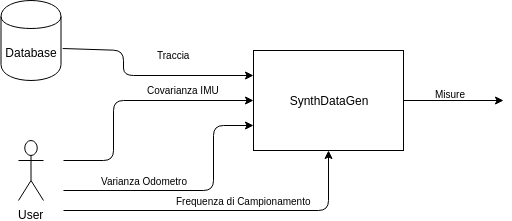
\includegraphics[width=0.7\linewidth]{img/SynthDataGen}
	\caption{Diagramma a blocchi \emph{SynthDataGen}}
	\label{fig:synthdatagen}
\end{figure}
\subsection{Injector}
Il \emph{faultload} \`e generato da uno specifico modulo (classe) di RTT.\\*
L'utente, attraverso l'interfaccia del software, \`e in grado di:
\begin{itemize}
	\item Sopprimere, per un arbitrario periodo di tempo, il canale di comunicazione tra i sensori e il modulo SFA;
	\item Alterare in modo casuale il contenuto dei messaggi trasmessi dai sensori al modulo SFA;
	\item Modificare i riferimenti geografici della traccia forniti in ingresso al modulo SFA.
\end{itemize}
\`E stato individuato questo \emph{fault model} considerando in primo luogo i requisiti del software. In particolare:
\begin{itemize}
		\item Ogni campionamento ricevuto dal sistema \textbf{deve} essere indicizzato;
		\item Il sistema \textbf{deve} scartare un campionamento quando questo viene ricevuto fuori ordine o il suo valore non \`e considerato accettabile in relazione ai valori ricevuti fino a quel momento;
		\item Quando il sistema scarta un campionamento, \textbf{deve} sostituirlo con una predizione del contenuto corretto, attraverso regressione lineare.
\end{itemize}
In secondo luogo, \`e opportuno considerare le tecnologie utilizzate. In 3.5.3 \`e stato dichiarato che la comunicazione tra i sensori e il modulo SFA, nel sistema reale, avviene utilizzando \texttt{UDP}.\\*
Questo protocollo di comunicazione non garantisce:
	\begin{itemize}
		\item La consegna dei messaggi;
		\item L'ordinamento dei messaggi;
		\item L'integrit\`a dei messaggi.
	\end{itemize}
\subsection{Monitor}
L'interfaccia utente di RTT fornisce una mappa su cui verr\`a marcata la posizione del treno durante gli esperimenti.\\*
I risultati intermedi prodotti da SFA sono mostrati su un grafico e riportati in un file di \emph{log}.\\*
\begin{figure}[h]
	\centering
	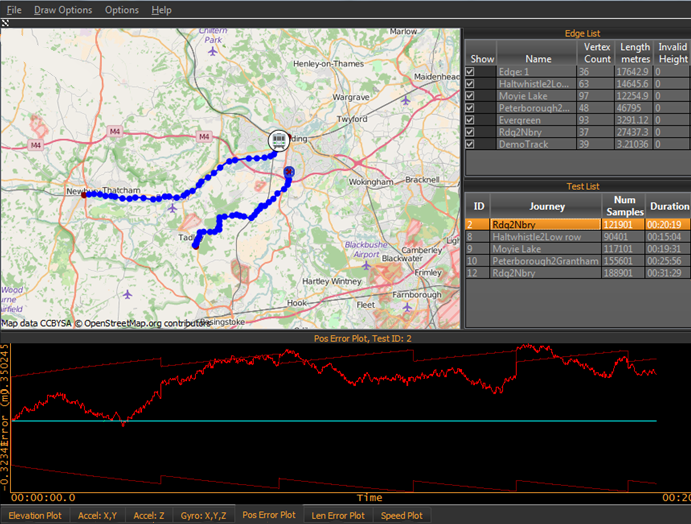
\includegraphics[width=0.7\linewidth]{img/rtthci2}
	\caption{Interfaccia utente di RTT}
	\label{fig:rtthci2}
\end{figure}
\subsection{Controller}
RTT integra al suo interno tutti gli elementi di una campagna di \emph{fault injection}, ed \`e pertanto in grado di controllarli.\\*
Per aumentare la \emph{reliability} dei risultati prodotti, RTT permette all'utente di definire il numero di ripetizioni da effettuare durante l'esecuzione di un esperimento.
\begin{figure}[h]
	\centering
	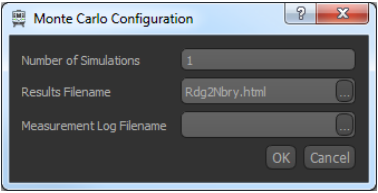
\includegraphics[width=0.7\linewidth]{img/imc}
	\caption{Controller RTT}
	\label{fig:montecarloconfig}
\end{figure}
Al termine di ciascun esperimento, RTT processa il file di \emph{log} prodotto dal modulo SFA e costruisce un report HTML contenente una sintesi dei risultati ottenuti (figura \ref{fig:rttreport}).
\begin{figure}
	\centering
	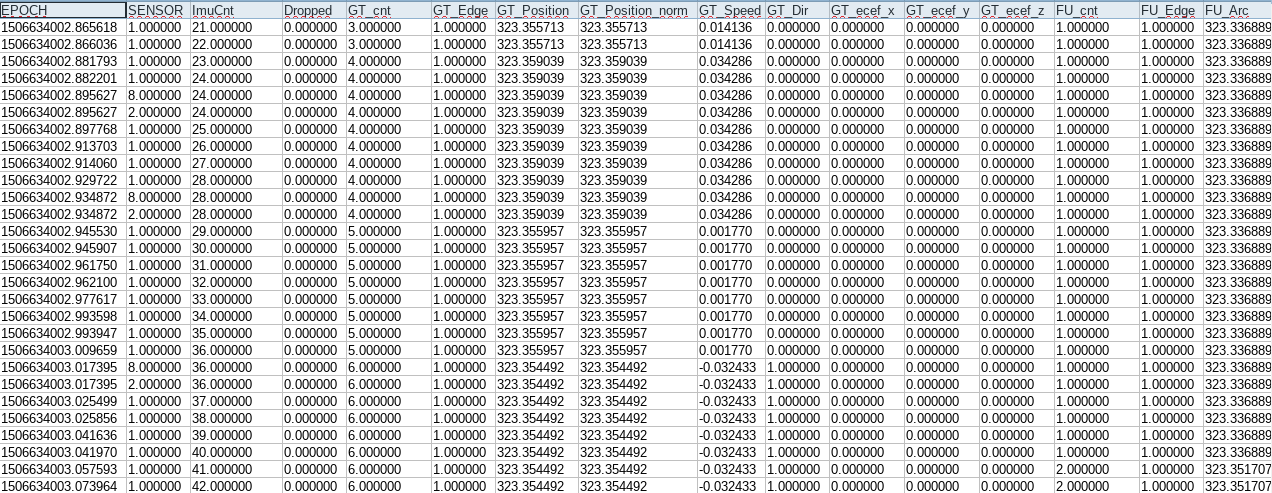
\includegraphics[width=\linewidth]{img/fusionlog}
	\caption{File di log}
	\label{fig:fusionlog}
\end{figure}
\section{Note sull'intrusivit\`a}
\`E noto dalla letteratura che un sistema di \emph{monitoring}, cos\`i come di \emph{fault injection}, deve essere il meno intrusivo possibile nei confronti del sistema monitorato.\\*
Il codice di \emph{SensorFusionLib} \`e stato instrumentato con delle \emph{software probe} che includono:
\begin{enumerate}
	\item La scrittura di un file di log che riporta l'evoluzione dello stato interno del software (figura \ref{fig:fusionlog});
	\item L'invio verso RTT dei calcoli intermedi compiuti dal software per stimare la posizione del treno. Questi sono:
	\begin{itemize}
		\item La stima dell'errore commesso sulla predizione delle coordinate geografiche del treno;
		\item La stima dell'errore commesso sulla predizione della progressiva chilometrica associata alle coordinate geografiche del treno;
		\item La stima della velocit\`a del treno;
		\item La stima dell'errore commesso sulla predizione della velocit\`a del treno.
	\end{itemize}
\end{enumerate}
Emergono alcune criticit\`a che \`e opportuno discutere.\\*
Le \emph{performance} di SFA potrebbero essere degradate dalla \emph{software probe} 1.\\*
Dover produrre un file di log implica la necessit\`a di accedere alla memoria di massa, e i tempi di accesso
possono essere di diversi ordini di grandezza superiori a quelli richiesti dall' accesso alla memoria centrale (o alla cache) imposto dalla \emph{software probe} 2.\\*
\begin{figure}[h]
	\centering
	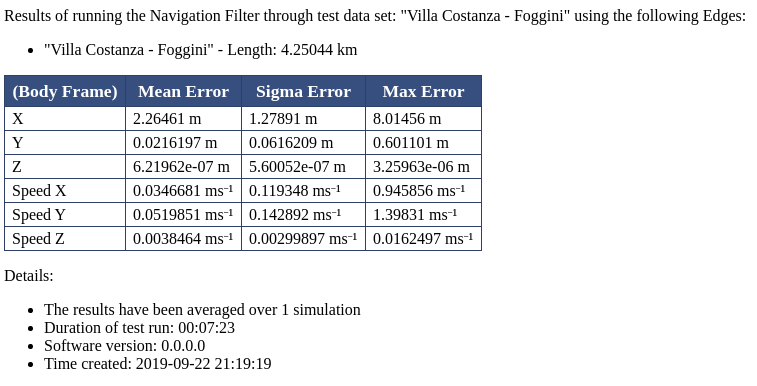
\includegraphics[width=0.7\linewidth]{img/rttreport}
	\caption{Report HTML prodotto da RTT}
	\label{fig:rttreport}
\end{figure}

